% $Header: /cvsroot/latex-beamer/latex-beamer/solutions/generic-talks/generic-ornate-15min-45min.en.tex,v 1.5 2007/01/28 20:48:23 tantau Exp $
\documentclass{beamer}
\mode<presentation>
{
 \usetheme{Warsaw}
 \usecolortheme{beaver}
 \usecolortheme{rose}
 \setbeamercovered{transparent}
}
\usepackage[english]{babel}
\usepackage[latin1]{inputenc}
\usepackage{graphicx}
\usepackage{times}
\usepackage[T1]{fontenc}
\usepackage{tabularx}

\title{Cloud Computing and the Ideal Mobile Platform}
\subtitle{How the advent of Cloud Computing might affect computers designed for
  mobile use}
\author{T.~Visher}
\institute[Chestnut Hill College]{Department of Computer Science\\
  Chestnut Hill College}
\date[Senior Seminar]{May 3rd, 2010 / Senior Seminar Presentation}
\subject{Cloud Computing and the Ideal Mobile Platform}

\pgfdeclareimage[height=0.75cm]{chc-logo}{redgrif}
\logo{\pgfuseimage{chc-logo}}

% Delete this, if you do not want the table of contents to pop up at
% the beginning of each subsection:
\AtBeginSubsection[]{
  \begin{frame}<beamer>{Outline}
    \tableofcontents[currentsection,currentsubsection]
  \end{frame}
}

\begin{document}

\begin{frame}
\titlepage
\end{frame}

\begin{frame}{Outline}
\tableofcontents[pausesections]
\end{frame}

% Since this a solution template for a generic talk, very little can
% be said about how it should be structured. However, the talk length
% of between 15min and 45min and the theme suggest that you stick to
% the following rules:

% - Exactly two or three sections (other than the summary).
% - At *most* three subsections per section.
% - Talk about 30s to 2min per frame. So there should be between about
%   15 and 30 frames, all told.

\section[Introduction]{Research Questions and Goals}

\begin{frame}{Goals}

\begin{itemize}
  \item A new mobile machine
  \item Prove Netbook/Notebook comparability
\end{itemize}

\end{frame}

\begin{frame}{Research Questions}
  \begin{itemize}
  \item Can the use of Cloud Services extend battery life?
  \item Are Netbooks and Notebooks favorably comparable \\ in the use of Cloud
    Services?
  \end{itemize}
\end{frame}

\section[Literature Review]{The Literature: The Internet and Computing}

\subsection{Thin Client Computing}

\begin{frame}{History}
  \begin{columns}
    \column{5cm}
      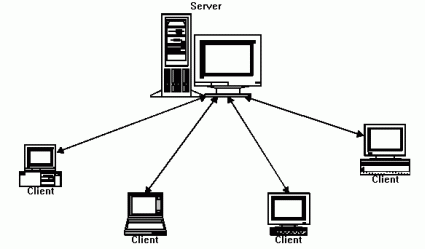
\includegraphics[width=5cm]{clientServer.png}
    \column{5cm}
      \begin{itemize}
      \item Client/Server
      \item Architecture
      \end{itemize}
  \end{columns}
\end{frame}

\begin{frame}{An Implementation: SLIM}
  \begin{columns}
    \column{5cm}
      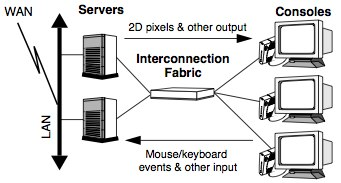
\includegraphics[width=5cm]{slimArchitecture.jpg}
    \column{5cm}
      \begin{itemize}
      \item Sun Microsystems (RIP)
      \item Architecture
      \item Rationale
      \end{itemize}
  \end{columns}
\end{frame}

\begin{frame}{Why?}
  \begin{columns}
    \column{5cm}
      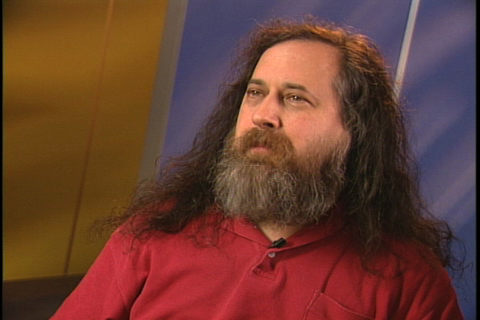
\includegraphics[width=5cm]{unixGeek.jpg}
    \column{5cm}
      \begin{itemize}
      \item Advantages
      \item Disadvantages
      \end{itemize}
  \end{columns}
\end{frame}

%% \begin{frame}{Current Applications}
%%   \begin{itemize}
%%   \item Medical Industry
%%   \end{itemize}
%% \end{frame}

\subsection{Cloud Computing}

\begin{frame}{History}
\begin{columns}
  \column{5cm}
    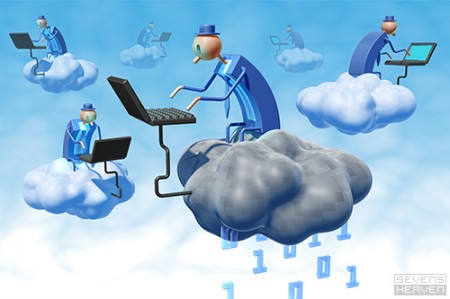
\includegraphics[width=5cm]{cloudComputing.jpg}
  \column{5cm}
    \begin{itemize}
    \item Roots
    \item Amazon
    \item Broadband
    \end{itemize}
\end{columns}
\end{frame}

\begin{frame}{Web 2.0}
  \begin{columns}
    \column{5cm}
      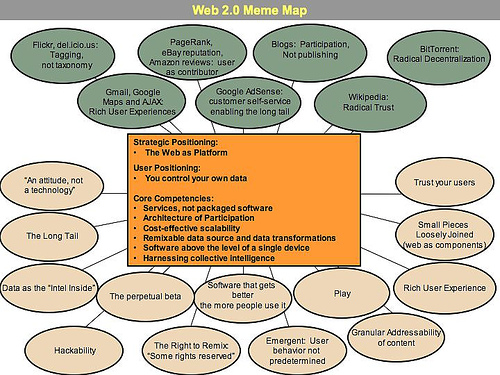
\includegraphics[width=5cm]{web20memeMap.jpg}
    \column{5cm}
      \begin{itemize}
      \item Tim O'Reilly
      \item Ethos
      \item Examples
      \end{itemize}
  \end{columns}
\end{frame}

\subsection{Lithium-Ion Batteries}

\begin{frame}{History}
  \begin{columns}
    \column{5cm}
      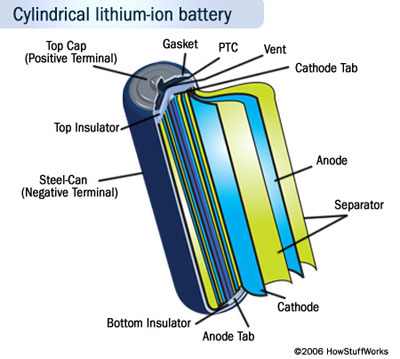
\includegraphics[width=5cm]{lionSummary.jpg}
    \column{5cm}
      \begin{itemize}
      \item Prior Art
      \item M. S. Whittingham
      \item Safety
      \end{itemize}
  \end{columns}
\end{frame}

\begin{frame}{How They Work}
  \begin{columns}
    \begin{column}{5cm}
      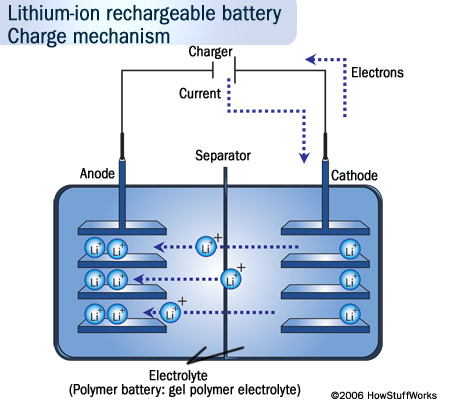
\includegraphics[width=5cm]{lionCharge.jpg}
    \end{column}
    \begin{column}{5cm}
      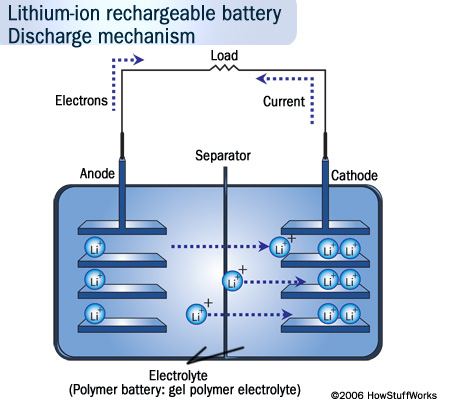
\includegraphics[width=5cm]{lionDischarge.jpg}
    \end{column}
  \end{columns}
\end{frame}

\begin{frame}{Future Research}
  \begin{itemize}
  \item Nano Technology
  \end{itemize}
\end{frame}

\subsection{Netbooks and Ultra-Mobile PCs}

\begin{frame}{History}
  \begin{columns}
    \column{5cm}
    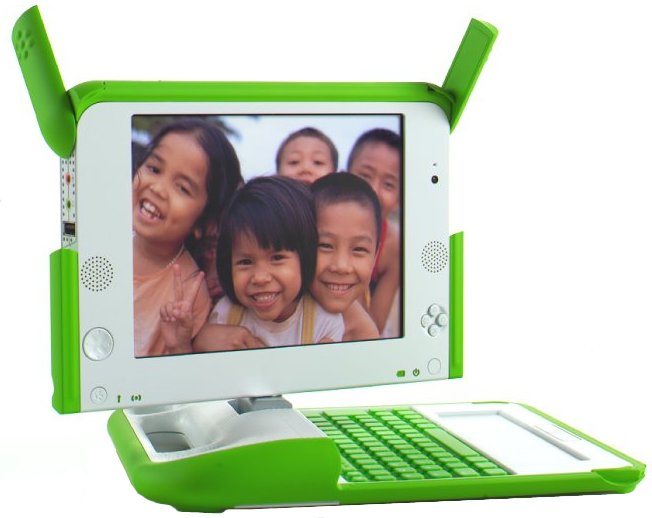
\includegraphics[width=5cm]{olpc.jpg}
    \column{5cm}
    \begin{itemize}
    \item Intel %% Paul Bergevin, 2008
    \item The First Netbook
    \item Drivers
    \end{itemize}
  \end{columns}
\end{frame}

\begin{frame}{Qualifications}
  \begin{columns}
    \column{5cm}
    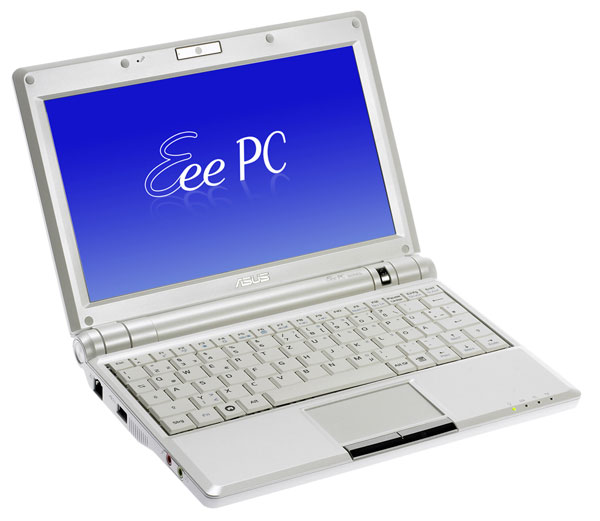
\includegraphics[width=5cm]{netbookSpecs.jpg}
    \column{5cm}
    \begin{itemize}
    \item Small
    \item Cheap
    \item Depend on the Net
    \end{itemize}
  \end{columns}
\end{frame}

\section[Research Project]{The Project: Mobile Hardware Using Cloud Services}

\subsection{Demand Management}

\begin{frame}{What Is Demand Management? }
  \begin{columns}
    \column{5cm}
      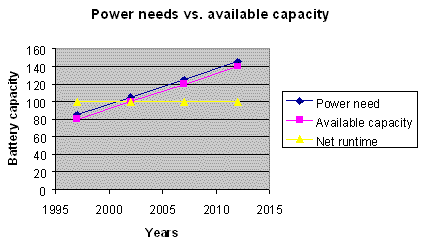
\includegraphics[width=5cm]{demandGraph.png}
    \column{5cm}
    \begin{itemize}
    \item It is\dots
    \item Why?
    \item Mr. Pogue
    \end{itemize}
  \end{columns}
\end{frame}

\begin{frame}{Notebooks+Demand Management}
  \begin{columns}
    \column{5cm}
      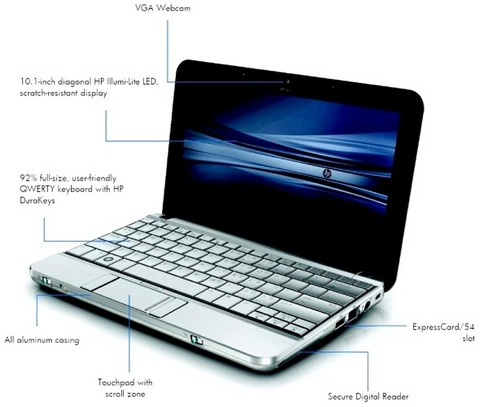
\includegraphics[width=5cm]{netbookDiagram.jpg}
    \column{5cm}
    \begin{itemize}
    \item Display Size
    \item Antenna Switch
    \item SSD
    \item CPU Throttling
    \item No Optical
    \end{itemize}
  \end{columns}
\end{frame}

\subsection[GDocs Spreadsheet Testing]{Google Docs Spreadsheet Torture Test}

\begin{frame}{Performance Testing}
  \begin{itemize}
  \item In General
  \end{itemize}
\end{frame}

\begin{frame}{Harware Specs}
  \resizebox{10cm}{!} {
  \begin{tabular}{| r | p{5cm} | p{5cm} |}
    \hline
                          & MacBook          & acer ASPIRE one   \\ \hline
    Processor Name        & Intel Core Duo   & Intel Atom N270   \\ \hline
    Processor Speed       & 1.83 GHz         & 1.60 GHz          \\ \hline
    Number Of Processors  & 1                & 1                 \\ \hline
    Total Number Of Cores & 2                & 1                 \\ \hline
    Operating System      & Mac OS X 10.6.3  & Windows XP HE SP3 \\ \hline
    \hline
  \end{tabular}
}
\end{frame}

\begin{frame}{Software Specs}
  \resizebox{10cm}{!} {
  \begin{tabular}{| r | p{5cm} | p{5cm} |}
    \hline
                                 & MacBook     & acer ASPIRE one \\ \hline
    Google Chrome                & 5.0.342.9                    & 4.1.249.1045 (42898)               \\ \hline
    OpenOffice.org               & 3.2.0 OOO320m12 (Build:9483) & 3.2.0 OOO320m12 (Build:9483)       \\
    \hline
  \end{tabular}
}
\end{frame}

\begin{frame}{The Process}
  \begin{itemize}
  \item Let the show begin\dots
  \end{itemize}
\end{frame}

\begin{frame}{Chrome/GDocs Performance}
  \begin{columns}
    \column{5cm}
    \resizebox{5cm}{!} {
    \begin{tabularx}{275pt}{| c | X | X | X |}
      \hline
      & \multicolumn{3}{c|}{MacBook steps in seconds} \\ \hline
      Run      & Step 1 & Step 2 & Step 3 \\ \hline
      1        & 8      & 2      & 30     \\ \hline
      2        & 7      & 3      & 17     \\ \hline
      3        & 5      & 4      & 24     \\ \hline
      4        & 6      & 3      & 23     \\ \hline
      5        & 6      & 2      & 29     \\ \hline
      6        & 4      & 5      & 28     \\ \hline
      7        & 5      & 2      & 30     \\ \hline
      8        & 6      & 2      & 19     \\ \hline
      9        & 6      & 3      & 20     \\ \hline
      10       & 7      & 3      & 23     \\ \hline
      Average  & 6      & 2.9    & 24.3   \\
      \hline
    \end{tabularx}
}
    \column{5cm}
    \resizebox{5cm}{!}{
    \begin{tabularx}{275pt}{| c | X | X | X |}
      \hline
      & \multicolumn{3}{c|}{ASPIRE steps in seconds} \\ \hline
      Run          & Step 1 & Step 2 & Step 3 \\ \hline
      1            & 8      & 2      & 17     \\ \hline
      2            & 7      & 3      & 30     \\ \hline
      3            & 5      & 2      & 23     \\ \hline
      4            & 6      & 3      & 30     \\ \hline
      5            & 7      & 4      & 20     \\ \hline
      6            & 9      & 5      & 24     \\ \hline
      7            & 3      & 2      & 29     \\ \hline
      8            & 10     & 3      & 22     \\ \hline
      9            & 6      & 3      & 30     \\ \hline
      10           & 7      & 4      & 23     \\ \hline
      Average      & 6.8    & 3.1    & 24.8   \\
      \hline
    \end{tabularx}
}
  \end{columns}
\end{frame}

\begin{frame}{OpenOffice.org Large Spreadsheet Performance}
  \begin{tabularx}{300pt}{| c | X | X |}
    \hline
    & \multicolumn{2}{c|}{Time to complete opening in seconds} \\ \hline
    Run               & Notebook & Netbook    \\ \hline
    1                 & 134      & 1800       \\ \hline
    2                 & 129      & 1738       \\ \hline
    3                 & 144      & 1721       \\ \hline
    4                 & 111      & 1983       \\ \hline
    5                 & 119      & 1699       \\ \hline
    6                 & 128      & 1738       \\ \hline
    7                 & 145      & 1715       \\ \hline
    8                 & 133      & 1817       \\ \hline
    9                 & 129      & 1876       \\ \hline
    10                & 125      & 1743       \\ \hline
    Average Times     & 129.7    & 1783       \\
    \hline
  \end{tabularx}
\end{frame}

\section*{Summary}

\begin{frame}{Summary}

\begin{itemize}
\item Netbook/Notebook performance is comparable
\item An ideal mobile platform?
\end{itemize}

\end{frame}

\end{document}
